\documentclass[a4paper]{article}\usepackage[]{graphicx}\usepackage[]{color}
%% maxwidth is the original width if it is less than linewidth
%% otherwise use linewidth (to make sure the graphics do not exceed the margin)
\makeatletter
\def\maxwidth{ %
  \ifdim\Gin@nat@width>\linewidth
    \linewidth
  \else
    \Gin@nat@width
  \fi
}
\makeatother

\definecolor{fgcolor}{rgb}{0.345, 0.345, 0.345}
\newcommand{\hlnum}[1]{\textcolor[rgb]{0.686,0.059,0.569}{#1}}%
\newcommand{\hlstr}[1]{\textcolor[rgb]{0.192,0.494,0.8}{#1}}%
\newcommand{\hlcom}[1]{\textcolor[rgb]{0.678,0.584,0.686}{\textit{#1}}}%
\newcommand{\hlopt}[1]{\textcolor[rgb]{0,0,0}{#1}}%
\newcommand{\hlstd}[1]{\textcolor[rgb]{0.345,0.345,0.345}{#1}}%
\newcommand{\hlkwa}[1]{\textcolor[rgb]{0.161,0.373,0.58}{\textbf{#1}}}%
\newcommand{\hlkwb}[1]{\textcolor[rgb]{0.69,0.353,0.396}{#1}}%
\newcommand{\hlkwc}[1]{\textcolor[rgb]{0.333,0.667,0.333}{#1}}%
\newcommand{\hlkwd}[1]{\textcolor[rgb]{0.737,0.353,0.396}{\textbf{#1}}}%
\let\hlipl\hlkwb

\usepackage{framed}
\makeatletter
\newenvironment{kframe}{%
 \def\at@end@of@kframe{}%
 \ifinner\ifhmode%
  \def\at@end@of@kframe{\end{minipage}}%
  \begin{minipage}{\columnwidth}%
 \fi\fi%
 \def\FrameCommand##1{\hskip\@totalleftmargin \hskip-\fboxsep
 \colorbox{shadecolor}{##1}\hskip-\fboxsep
     % There is no \\@totalrightmargin, so:
     \hskip-\linewidth \hskip-\@totalleftmargin \hskip\columnwidth}%
 \MakeFramed {\advance\hsize-\width
   \@totalleftmargin\z@ \linewidth\hsize
   \@setminipage}}%
 {\par\unskip\endMakeFramed%
 \at@end@of@kframe}
\makeatother

\definecolor{shadecolor}{rgb}{.97, .97, .97}
\definecolor{messagecolor}{rgb}{0, 0, 0}
\definecolor{warningcolor}{rgb}{1, 0, 1}
\definecolor{errorcolor}{rgb}{1, 0, 0}
\newenvironment{knitrout}{}{} % an empty environment to be redefined in TeX

\usepackage{alltt}

\usepackage{amsmath, amsfonts, amssymb}
\IfFileExists{upquote.sty}{\usepackage{upquote}}{}
\begin{document}




\section{Discrete time}
  Suppose you have a difference equation
	\begin{equation}
		\label{eq:discrete}
		x_{t+1} = f(x_t),
	\end{equation}
	where $t\in \mathbb{N}$. The system does not change iff $x_{t+1} = x_t = x^*$. The resulting \emph{equilibrium} or \emph{fixed} points $x^*$ are determined by the intersection of the bisectrix and $f$, that is the criterion:
	\begin{equation}
		\label{eq:5}
		x^*=f(x^*).
	\end{equation}
	A fixed point can be either attractive, repelling, or neutral. This can be determined from the derivative $f'$ at the fixed point. One finds that {\bf $x^*$ is attractive if $|f'(x^*)| < 1$, and $x^*$ is repelling if $|f'(x^*)|>1$}. To understand these criteria, suppose we are at a position close to the fixed point, $x_t = x^* + \epsilon_t$. We analyze the evolution of the distance $\epsilon_t$. As $\epsilon_t$ is small, we use a Taylor expansion
	\begin{equation}
		\label{eq:4}
		\epsilon_{t+1} = f(x^*+\epsilon_t) - f(x^*) \approx f'(x^*) \epsilon_t.
	\end{equation}
	From this equation we see that the increment will only decrease if $|f'(x^*)|<1$, which is exactly the criterion for stability.
	
	\subsection{An example}
	Suppose we have $f(x) = 5x^2(1-x)$. Solving $f(x) = x$ yields the fixed points $x_1^*=0$, $x_2^* = \frac{1}{2} - \frac{\sqrt{5}}{10} \approx 0.28$, and $x^*_3 = \frac{1}{2} + \frac{\sqrt{5}}{10} \approx 0.72$. As shown below, however, only $x^*_1$ and $x^*_3$ are attractive.
	\begin{center}
		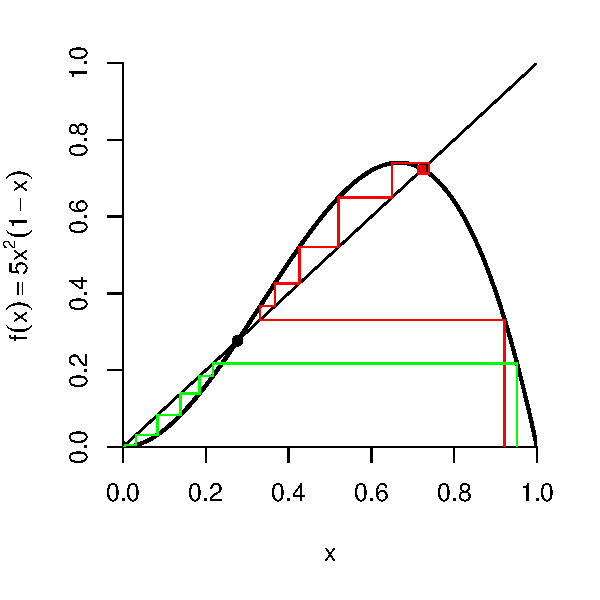
\includegraphics[width=6.66cm]{tutorial-p2.pdf}
	\end{center}


\begin{knitrout}
\definecolor{shadecolor}{rgb}{0.969, 0.969, 0.969}\color{fgcolor}\begin{kframe}
\begin{alltt}
\hlstd{steps} \hlkwb{<-} \hlnum{100}
\hlstd{xs} \hlkwb{<-} \hlkwd{rep}\hlstd{(}\hlnum{0}\hlstd{, steps)}
\hlstd{xs[}\hlnum{1}\hlstd{]} \hlkwb{<-} \hlnum{0.95}  \hlcom{# initial condition}
\hlkwa{for} \hlstd{(ii} \hlkwa{in} \hlnum{2}\hlopt{:}\hlstd{steps) \{}
    \hlstd{xs[ii]} \hlkwb{<-} \hlnum{5} \hlopt{*} \hlstd{xs[ii} \hlopt{-} \hlnum{1}\hlstd{]}\hlopt{^}\hlnum{2} \hlopt{*} \hlstd{(}\hlnum{1} \hlopt{-} \hlstd{xs[ii} \hlopt{-} \hlnum{1}\hlstd{])}
\hlstd{\}}
\end{alltt}
\end{kframe}
\end{knitrout}

\begin{knitrout}
\definecolor{shadecolor}{rgb}{0.969, 0.969, 0.969}\color{fgcolor}\begin{kframe}
\begin{alltt}
\hlkwd{par}\hlstd{(}\hlkwc{mar} \hlstd{=} \hlkwd{c}\hlstd{(}\hlnum{4}\hlstd{,} \hlnum{4}\hlstd{,} \hlnum{0.5}\hlstd{,} \hlnum{0.5}\hlstd{))}
\hlkwd{par}\hlstd{(}\hlkwc{mgp} \hlstd{=} \hlkwd{c}\hlstd{(}\hlnum{2.5}\hlstd{,} \hlnum{1}\hlstd{,} \hlnum{0}\hlstd{))}
\hlkwd{par}\hlstd{(}\hlkwc{cex.lab} \hlstd{=} \hlnum{1.25}\hlstd{)}
\hlkwd{plot}\hlstd{(xs,} \hlkwc{xlab} \hlstd{=} \hlstr{"step"}\hlstd{,} \hlkwc{ylab} \hlstd{=} \hlstr{"x"}\hlstd{,} \hlkwc{main} \hlstd{=} \hlstr{""}\hlstd{,} \hlkwc{col} \hlstd{=} \hlstr{"dodgerblue"}\hlstd{,}
    \hlkwc{pch} \hlstd{=} \hlnum{20}\hlstd{,} \hlkwc{ylim} \hlstd{=} \hlkwd{c}\hlstd{(}\hlnum{0}\hlstd{,} \hlnum{1}\hlstd{))}
\hlkwd{abline}\hlstd{(}\hlkwc{h} \hlstd{=} \hlnum{0}\hlstd{,} \hlkwc{col} \hlstd{=} \hlstr{"#ff8c00"}\hlstd{,} \hlkwc{lwd} \hlstd{=} \hlnum{2}\hlstd{)}
\end{alltt}
\end{kframe}

{\centering 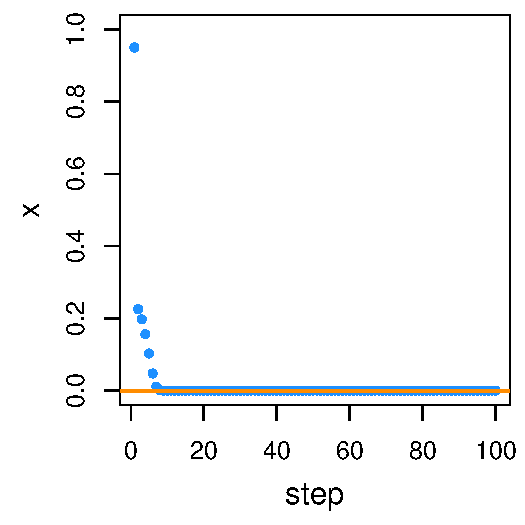
\includegraphics[width=\maxwidth]{figure/minimal-unnamed-chunk-2-1} 

}



\end{knitrout}

\begin{knitrout}
\definecolor{shadecolor}{rgb}{0.969, 0.969, 0.969}\color{fgcolor}\begin{kframe}
\begin{alltt}
\hlstd{xs[}\hlnum{1}\hlstd{]} \hlkwb{<-} \hlnum{0.9}  \hlcom{# initial condition}
\hlkwa{for} \hlstd{(ii} \hlkwa{in} \hlnum{2}\hlopt{:}\hlstd{steps) \{}
    \hlstd{xs[ii]} \hlkwb{<-} \hlnum{5} \hlopt{*} \hlstd{xs[ii} \hlopt{-} \hlnum{1}\hlstd{]}\hlopt{^}\hlnum{2} \hlopt{*} \hlstd{(}\hlnum{1} \hlopt{-} \hlstd{xs[ii} \hlopt{-} \hlnum{1}\hlstd{])}
\hlstd{\}}
\end{alltt}
\end{kframe}
\end{knitrout}


\begin{knitrout}
\definecolor{shadecolor}{rgb}{0.969, 0.969, 0.969}\color{fgcolor}\begin{kframe}
\begin{alltt}
\hlkwd{plot}\hlstd{(xs,} \hlkwc{xlab} \hlstd{=} \hlstr{"step"}\hlstd{,} \hlkwc{ylab} \hlstd{=} \hlstr{"x"}\hlstd{,} \hlkwc{main} \hlstd{=} \hlstr{""}\hlstd{,} \hlkwc{col} \hlstd{=} \hlstr{"dodgerblue"}\hlstd{,}
    \hlkwc{pch} \hlstd{=} \hlnum{20}\hlstd{,} \hlkwc{ylim} \hlstd{=} \hlkwd{c}\hlstd{(}\hlnum{0}\hlstd{,} \hlnum{1}\hlstd{))}
\hlkwd{abline}\hlstd{(}\hlkwc{h} \hlstd{=} \hlnum{1}\hlopt{/}\hlnum{2} \hlopt{+} \hlkwd{sqrt}\hlstd{(}\hlnum{5}\hlstd{)}\hlopt{/}\hlnum{10}\hlstd{,} \hlkwc{col} \hlstd{=} \hlstr{"#ff8c00"}\hlstd{,} \hlkwc{lwd} \hlstd{=} \hlnum{2}\hlstd{)}
\end{alltt}
\end{kframe}

{\centering 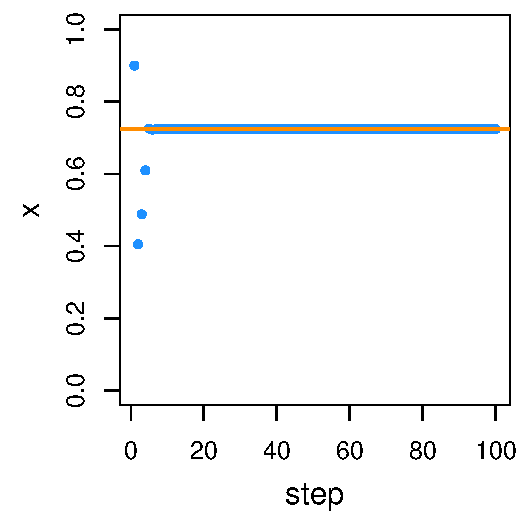
\includegraphics[width=\maxwidth]{figure/minimal-unnamed-chunk-4-1} 

}



\end{knitrout}

On the Poincar\'e plot of $x_t$ against $x_{t-1}$ we can trace the path to the stable fixed point

\begin{knitrout}
\definecolor{shadecolor}{rgb}{0.969, 0.969, 0.969}\color{fgcolor}\begin{kframe}
\begin{alltt}
\hlstd{xstm1} \hlkwb{<-} \hlstd{xs[}\hlopt{-}\hlkwd{length}\hlstd{(xs)]}
\hlstd{xst} \hlkwb{<-} \hlstd{xs[}\hlopt{-}\hlnum{1}\hlstd{]}
\hlkwd{plot}\hlstd{(xstm1, xst,} \hlkwc{xlab} \hlstd{=} \hlkwd{expression}\hlstd{(x[t} \hlopt{-} \hlnum{1}\hlstd{]),} \hlkwc{ylab} \hlstd{=} \hlkwd{expression}\hlstd{(x[t]),}
    \hlkwc{main} \hlstd{=} \hlstr{""}\hlstd{,} \hlkwc{col} \hlstd{=} \hlstr{"dodgerblue"}\hlstd{,} \hlkwc{pch} \hlstd{=} \hlnum{20}\hlstd{,} \hlkwc{xlim} \hlstd{=} \hlkwd{c}\hlstd{(}\hlnum{0}\hlstd{,} \hlnum{1}\hlstd{),} \hlkwc{ylim} \hlstd{=} \hlkwd{c}\hlstd{(}\hlnum{0}\hlstd{,}
        \hlnum{1}\hlstd{))}
\hlkwd{lines}\hlstd{(xstm1, xst,} \hlkwc{col} \hlstd{=} \hlstr{"dodgerblue"}\hlstd{,} \hlkwc{lwd} \hlstd{=} \hlnum{0.5}\hlstd{)}
\hlkwd{abline}\hlstd{(}\hlkwc{b} \hlstd{=} \hlnum{1}\hlstd{,} \hlkwc{a} \hlstd{=} \hlnum{0}\hlstd{,} \hlkwc{col} \hlstd{=} \hlstr{"#ff8c00"}\hlstd{,} \hlkwc{lwd} \hlstd{=} \hlnum{2}\hlstd{)}
\end{alltt}
\end{kframe}

{\centering 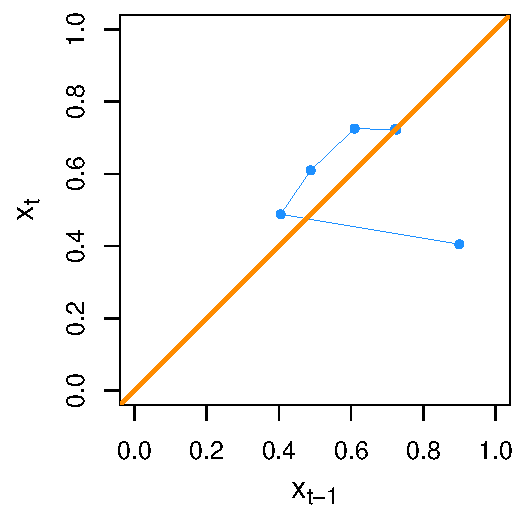
\includegraphics[width=\maxwidth]{figure/minimal-unnamed-chunk-5-1} 

}



\end{knitrout}

\section{Continuous time: Single variable models}
  We consider a dynamical system which is described by the single function of time $x$. The quantity $x(t)$ represents the value of $x$ as a function of the continuous time variable $t$.  The dynamical behaviour of the system is described by the differential equation
	\begin{equation}
		\frac{dx}{dt} = f(x(t)).
	\end{equation}
	
	\subsection{Finding equilibrium points}
	An equilibrium point of the system is a value for the variable such that the state of the system does not change any more. The condition for the equilibrium is that
	\begin{equation*}
		\dot{x} = \frac{dx}{dt} =0.
	\end{equation*}
	Thus, one has to solve the equation
	\begin{equation}
		\label{equil}
		f(x) = 0.
	\end{equation}
	We denote the equilibrium point by $x^*$. Note that the equation \ref{equil} can in general have more than one solution, each corresponding to a different  equilibrium.
	
	\subsection{Determining the stability of equilibria}
	If we plug the equilibrium point in the equation describing the dynamics of the system, we will find that it will not change. But what if the system starts from a point close but not exactly equal to an equilibrium point? This is the subject of stability analysis.
	
	Let's suppose that the system at time $t$ is in a position $x(t) = x^* + \varepsilon(t)$, \emph{i.e.}\ displaced by a quantity $\varepsilon$ from an equilibrium point. How will the system evolve? Will the displacement increase or decrease? To answer this question, we can write the evolution of the displacement $\varepsilon(t)$
	\begin{equation}
		\frac{d\varepsilon}{dt} = \frac{d}{dt}(x(t)-x^*) = f(x(t)) = f(x^* + \varepsilon(t)).
	\end{equation}
	Taking the Taylor expansion of  $f(x)$ around the point $x^*$ we can write
	\begin{equation}
		\frac{d\varepsilon}{dt} = f(x^*) + \underbrace{\frac{df}{dx}|_{x=x^*}}_{= r} \varepsilon(t) = 0 + r \varepsilon(t).
	\end{equation}
	Solving this differential equation we obtain
	\begin{equation}
		\varepsilon(t) = e^{rt}\varepsilon(t=0).
	\end{equation}
	It is easy to see that {\bf the condition for the stability of the equilibrium is $r = \frac{df}{dx}|_{x=x^*}  < 0$}.

	\subsection{An example}
	Consider the case $f(x)=3x(x-1)(x-2)$. The third degree polynomial $f$ has three zero. Thus, the fixed points are given by $x_1^*=0$, $x_2^*=1$, $x_3^*=2$.
	\begin{center}
		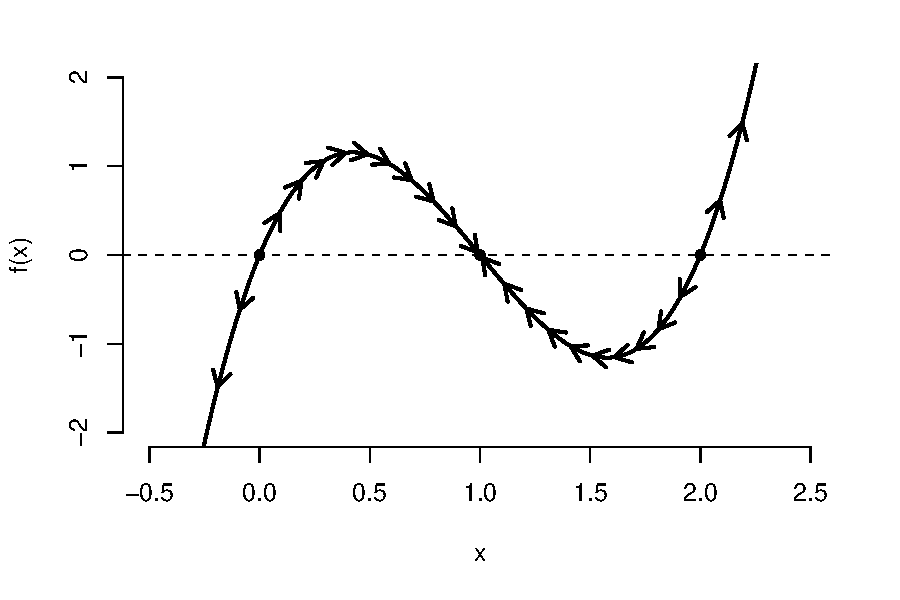
\includegraphics[width=10cm]{tutorial-p1.pdf}
	\end{center}
	
	Which of them are stable? The derivative of $f$ is $f'(x)=3(x-1)(x-2) + 3x(x-2) + 3x(x-1)$. We find that $f'(x_1^*)=6 $, $f'(x_2^*)=-3$, and $f'(x_3^*)=6$. That is $x_1^*$ and $x_3^*$ are unstable, and $x_2^*$ is stable ($f'(x_2^*) < 0$).

\begin{knitrout}
\definecolor{shadecolor}{rgb}{0.969, 0.969, 0.969}\color{fgcolor}\begin{kframe}
\begin{alltt}
\hlkwd{library}\hlstd{(deSolve)}
\hlstd{parms} \hlkwb{<-} \hlkwd{c}\hlstd{()}
\hlstd{my.atol} \hlkwb{<-} \hlkwd{c}\hlstd{(}\hlnum{1e-06}\hlstd{)}
\hlstd{times} \hlkwb{<-} \hlkwd{c}\hlstd{(}\hlnum{0}\hlopt{:}\hlnum{100}\hlstd{)}\hlopt{/}\hlnum{25}
\hlstd{sdiffeqns} \hlkwb{<-} \hlkwa{function}\hlstd{(}\hlkwc{t}\hlstd{,} \hlkwc{s}\hlstd{,} \hlkwc{parms}\hlstd{) \{}
    \hlstd{sd1} \hlkwb{<-} \hlnum{3} \hlopt{*} \hlstd{s[}\hlnum{1}\hlstd{]} \hlopt{*} \hlstd{(s[}\hlnum{1}\hlstd{]} \hlopt{-} \hlnum{1}\hlstd{)} \hlopt{*} \hlstd{(s[}\hlnum{1}\hlstd{]} \hlopt{-} \hlnum{2}\hlstd{)}
    \hlkwd{list}\hlstd{(}\hlkwd{c}\hlstd{(sd1))}
\hlstd{\}}
\end{alltt}
\end{kframe}
\end{knitrout}

We can check this by numerically integrating the differential equation starting at $x^{*}\pm\epsilon$

\begin{knitrout}
\definecolor{shadecolor}{rgb}{0.969, 0.969, 0.969}\color{fgcolor}\begin{kframe}
\begin{alltt}
\hlstd{initconds} \hlkwb{<-} \hlkwd{c}\hlstd{(}\hlnum{0} \hlopt{-} \hlnum{1e-06}\hlstd{)}  \hlcom{# just below 0}
\hlstd{out0m} \hlkwb{<-} \hlkwd{lsoda}\hlstd{(initconds, times, sdiffeqns,} \hlkwc{rtol} \hlstd{=} \hlnum{1e-10}\hlstd{,} \hlkwc{atol} \hlstd{= my.atol)}
\end{alltt}
\begin{verbatim}
DLSODA-  Warning..Internal T (=R1) and H (=R2) are
      such that in the machine, T + H = T on the next step  
     (H = step size). Solver will continue anyway.
In above message, R1 = 2.18389, R2 = 2.00327e-16
 
DLSODA-  Warning..Internal T (=R1) and H (=R2) are
      such that in the machine, T + H = T on the next step  
     (H = step size). Solver will continue anyway.
In above message, R1 = 2.18389, R2 = 2.00327e-16
 
DLSODA-  Warning..Internal T (=R1) and H (=R2) are
      such that in the machine, T + H = T on the next step  
     (H = step size). Solver will continue anyway.
In above message, R1 = 2.18389, R2 = 2.00327e-16
 
DLSODA-  Warning..Internal T (=R1) and H (=R2) are
      such that in the machine, T + H = T on the next step  
     (H = step size). Solver will continue anyway.
In above message, R1 = 2.18389, R2 = 2.00327e-16
 
DLSODA-  Warning..Internal T (=R1) and H (=R2) are
      such that in the machine, T + H = T on the next step  
     (H = step size). Solver will continue anyway.
In above message, R1 = 2.18389, R2 = 2.00327e-16
 
DLSODA-  Warning..Internal T (=R1) and H (=R2) are
      such that in the machine, T + H = T on the next step  
     (H = step size). Solver will continue anyway.
In above message, R1 = 2.18389, R2 = 2.00327e-16
 
DLSODA-  Warning..Internal T (=R1) and H (=R2) are
      such that in the machine, T + H = T on the next step  
     (H = step size). Solver will continue anyway.
In above message, R1 = 2.18389, R2 = 2.00327e-16
 
DLSODA-  Warning..Internal T (=R1) and H (=R2) are
      such that in the machine, T + H = T on the next step  
     (H = step size). Solver will continue anyway.
In above message, R1 = 2.18389, R2 = 2.00327e-16
 
DLSODA-  Warning..Internal T (=R1) and H (=R2) are
      such that in the machine, T + H = T on the next step  
     (H = step size). Solver will continue anyway.
In above message, R1 = 2.18389, R2 = 1.64605e-16
 
DLSODA-  Warning..Internal T (=R1) and H (=R2) are
      such that in the machine, T + H = T on the next step  
     (H = step size). Solver will continue anyway.
In above message, R1 = 2.18389, R2 = 1.64605e-16
 
DLSODA-  Above warning has been issued I1 times.  
     It will not be issued again for this problem.
In above message, I1 = 10
 
DLSODA-  At current T (=R1), MXSTEP (=I1) steps   
      taken on this call before reaching TOUT     
In above message, I1 = 5000
 
In above message, R1 = 2.18389
 
\end{verbatim}
\begin{alltt}
\hlstd{initconds} \hlkwb{<-} \hlkwd{c}\hlstd{(}\hlnum{0} \hlopt{+} \hlnum{1e-06}\hlstd{)}  \hlcom{# just above 0}
\hlstd{out0p} \hlkwb{<-} \hlkwd{lsoda}\hlstd{(initconds, times, sdiffeqns,} \hlkwc{rtol} \hlstd{=} \hlnum{1e-10}\hlstd{,} \hlkwc{atol} \hlstd{= my.atol)}
\hlstd{initconds} \hlkwb{<-} \hlkwd{c}\hlstd{(}\hlnum{1} \hlopt{-} \hlnum{1e-06}\hlstd{)}  \hlcom{# just below 1}
\hlstd{out1m} \hlkwb{<-} \hlkwd{lsoda}\hlstd{(initconds, times, sdiffeqns,} \hlkwc{rtol} \hlstd{=} \hlnum{1e-10}\hlstd{,} \hlkwc{atol} \hlstd{= my.atol)}
\hlstd{initconds} \hlkwb{<-} \hlkwd{c}\hlstd{(}\hlnum{1} \hlopt{+} \hlnum{1e-06}\hlstd{)}  \hlcom{# just above 1}
\hlstd{out1p} \hlkwb{<-} \hlkwd{lsoda}\hlstd{(initconds, times, sdiffeqns,} \hlkwc{rtol} \hlstd{=} \hlnum{1e-10}\hlstd{,} \hlkwc{atol} \hlstd{= my.atol)}
\hlstd{initconds} \hlkwb{<-} \hlkwd{c}\hlstd{(}\hlnum{2} \hlopt{-} \hlnum{1e-06}\hlstd{)}  \hlcom{# just below 2}
\hlstd{out2m} \hlkwb{<-} \hlkwd{lsoda}\hlstd{(initconds, times, sdiffeqns,} \hlkwc{rtol} \hlstd{=} \hlnum{1e-10}\hlstd{,} \hlkwc{atol} \hlstd{= my.atol)}
\hlstd{initconds} \hlkwb{<-} \hlkwd{c}\hlstd{(}\hlnum{2} \hlopt{+} \hlnum{1e-06}\hlstd{)}  \hlcom{# just above 2}
\hlstd{out2p} \hlkwb{<-} \hlkwd{lsoda}\hlstd{(initconds, times, sdiffeqns,} \hlkwc{rtol} \hlstd{=} \hlnum{1e-10}\hlstd{,} \hlkwc{atol} \hlstd{= my.atol)}
\end{alltt}
\begin{verbatim}
DLSODA-  Warning..Internal T (=R1) and H (=R2) are
      such that in the machine, T + H = T on the next step  
     (H = step size). Solver will continue anyway.
In above message, R1 = 2.18389, R2 = 2.00258e-16
 
DLSODA-  Warning..Internal T (=R1) and H (=R2) are
      such that in the machine, T + H = T on the next step  
     (H = step size). Solver will continue anyway.
In above message, R1 = 2.18389, R2 = 2.00258e-16
 
DLSODA-  Warning..Internal T (=R1) and H (=R2) are
      such that in the machine, T + H = T on the next step  
     (H = step size). Solver will continue anyway.
In above message, R1 = 2.18389, R2 = 2.00258e-16
 
DLSODA-  Warning..Internal T (=R1) and H (=R2) are
      such that in the machine, T + H = T on the next step  
     (H = step size). Solver will continue anyway.
In above message, R1 = 2.18389, R2 = 2.00258e-16
 
DLSODA-  Warning..Internal T (=R1) and H (=R2) are
      such that in the machine, T + H = T on the next step  
     (H = step size). Solver will continue anyway.
In above message, R1 = 2.18389, R2 = 2.00258e-16
 
DLSODA-  Warning..Internal T (=R1) and H (=R2) are
      such that in the machine, T + H = T on the next step  
     (H = step size). Solver will continue anyway.
In above message, R1 = 2.18389, R2 = 2.00258e-16
 
DLSODA-  Warning..Internal T (=R1) and H (=R2) are
      such that in the machine, T + H = T on the next step  
     (H = step size). Solver will continue anyway.
In above message, R1 = 2.18389, R2 = 2.00258e-16
 
DLSODA-  Warning..Internal T (=R1) and H (=R2) are
      such that in the machine, T + H = T on the next step  
     (H = step size). Solver will continue anyway.
In above message, R1 = 2.18389, R2 = 2.00258e-16
 
DLSODA-  Warning..Internal T (=R1) and H (=R2) are
      such that in the machine, T + H = T on the next step  
     (H = step size). Solver will continue anyway.
In above message, R1 = 2.18389, R2 = 1.64549e-16
 
DLSODA-  Warning..Internal T (=R1) and H (=R2) are
      such that in the machine, T + H = T on the next step  
     (H = step size). Solver will continue anyway.
In above message, R1 = 2.18389, R2 = 1.64549e-16
 
DLSODA-  Above warning has been issued I1 times.  
     It will not be issued again for this problem.
In above message, I1 = 10
 
DLSODA-  At current T (=R1), MXSTEP (=I1) steps   
      taken on this call before reaching TOUT     
In above message, I1 = 5000
 
In above message, R1 = 2.18389
 
\end{verbatim}
\end{kframe}
\end{knitrout}

\begin{knitrout}
\definecolor{shadecolor}{rgb}{0.969, 0.969, 0.969}\color{fgcolor}\begin{kframe}
\begin{alltt}
\hlkwd{plot}\hlstd{(out0p,} \hlkwc{xlab} \hlstd{=} \hlstr{"time"}\hlstd{,} \hlkwc{ylab} \hlstd{=} \hlstr{"x"}\hlstd{,} \hlkwc{main} \hlstd{=} \hlstr{""}\hlstd{,} \hlkwc{col} \hlstd{=} \hlstr{"dodgerblue"}\hlstd{,}
    \hlkwc{lty} \hlstd{=} \hlnum{1}\hlstd{,} \hlkwc{lwd} \hlstd{=} \hlnum{2}\hlstd{,} \hlkwc{ylim} \hlstd{=} \hlkwd{c}\hlstd{(}\hlopt{-}\hlnum{2}\hlstd{,} \hlnum{4}\hlstd{),} \hlkwc{xlim} \hlstd{=} \hlkwd{c}\hlstd{(}\hlnum{0}\hlstd{,} \hlnum{4}\hlstd{))}
\hlkwd{lines}\hlstd{(out0m,} \hlkwc{col} \hlstd{=} \hlstr{"#ff8c00"}\hlstd{,} \hlkwc{lty} \hlstd{=} \hlnum{3}\hlstd{,} \hlkwc{lwd} \hlstd{=} \hlnum{3}\hlstd{)}
\hlkwd{lines}\hlstd{(out2m,} \hlkwc{col} \hlstd{=} \hlstr{"dodgerblue"}\hlstd{,} \hlkwc{lty} \hlstd{=} \hlnum{1}\hlstd{,} \hlkwc{lwd} \hlstd{=} \hlnum{2}\hlstd{)}
\hlkwd{lines}\hlstd{(out2p,} \hlkwc{col} \hlstd{=} \hlstr{"#ff8c00"}\hlstd{,} \hlkwc{lty} \hlstd{=} \hlnum{3}\hlstd{,} \hlkwc{lwd} \hlstd{=} \hlnum{3}\hlstd{)}
\hlkwd{lines}\hlstd{(out1m,} \hlkwc{col} \hlstd{=} \hlstr{"#68228b"}\hlstd{,} \hlkwc{lty} \hlstd{=} \hlnum{2}\hlstd{,} \hlkwc{lwd} \hlstd{=} \hlnum{2}\hlstd{)}
\hlkwd{lines}\hlstd{(out1p,} \hlkwc{col} \hlstd{=} \hlstr{"#cd2626"}\hlstd{,} \hlkwc{lty} \hlstd{=} \hlnum{3}\hlstd{,} \hlkwc{lwd} \hlstd{=} \hlnum{3}\hlstd{)}
\end{alltt}
\end{kframe}

{\centering 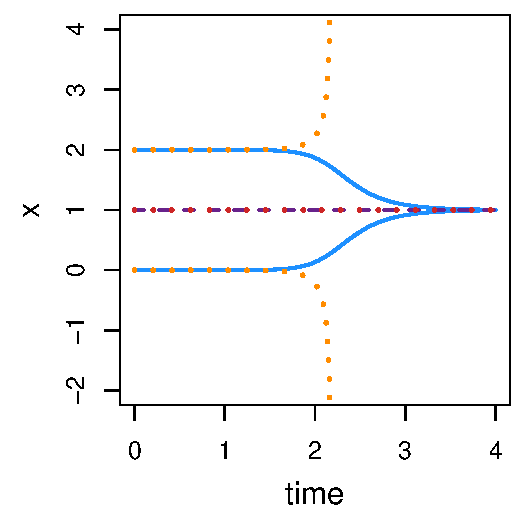
\includegraphics[width=\maxwidth]{figure/minimal-unnamed-chunk-8-1} 

}



\end{knitrout}






\end{document}
